\documentclass[11pt,pdf,aspectratio=129]{beamer}
\usepackage{bibentry}
\usepackage{graphicx} % Allows including images
\usepackage{booktabs} % Allows the use of \toprule, 
\usepackage{array}
\usepackage{wrapfig}
\usepackage{graphics}
\usepackage{graphicx}
\usepackage{amsfonts}
\usepackage{amssymb}
\usepackage{amsthm}
\usepackage{textcomp}
% \usepackage{enumitem}
\usepackage{bibentry}
\usepackage{graphicx} % Allows including images
\usepackage{booktabs} % Allows the use of \toprule, 
% \usepackage[nottoc]{tocbibind}
\usepackage{threeparttable}
\usepackage{natbib}
\usepackage{mathrsfs}
\usepackage[nospace]{varioref}	
\usepackage{cleveref}

\setlength{\parskip}{\baselineskip} 
\graphicspath{{./../Figures}}
\setlength\itemsep{2em}

\usepackage{caption}
\usepackage{subcaption}


\title{Verifying HANK}
\subtitle{Evidence from size-persistence tradeoff.}   
\author{\href{mailto://avlasov@nes.ru}{Alexander Vlasov}} 
\institute{NES}
\usetheme{Madrid}
% \usecolortheme{}

% \AtBeginSection{
% 	\begin{frame}
% 		\frametitle{Contents}
% 		\tableofcontents[currentsection]
% 	\end{frame}
% }

\begin{document}

\begin{frame}[fragile]
    \titlepage
\end{frame}


\section{Research question}
\begin{frame}
    \frametitle{Contents}
    \tableofcontents[currentsection]
\end{frame}


\begin{frame}\frametitle{What is HANK?}
    \[\text{NK}= \text{New Keynesian}=\text{Monetary Policy is not Neutral}\]
    \[\text{RANK}=\text{Representative Agent}+\text{NK}\]
    \[\text{TANK}=\text{Two-Agent}\footnote{Sometimes referred as Spender-Saver Model}+\text{NK}=\text{One agent is Spender, one is Saver}+\text{NK}\]
    \[\text{HANK}\footnote{The version by \citet{KMV2018}}=\text{Heterogeneous Agent}+\text{{NK}}=\text{Heterogenity in saving portfolio}+\text{NK}
    \]
    
    \footnotetext{See \citet{Gali2018} for review.}
    
    \end{frame}
    

\begin{frame}\frametitle{Outcomes of \citet{KMV2018} model}
    \citet{KMV2018} HANK model outcomes:
    \begin{enumerate}
        \item \textbf{Size-Persistence trade-off:} Cumulative elasticity of aggregate consumption declines with the increase in autocorrelation of monetary shock in a nonlinear manner.
        \item \textbf{Inflation-Output Tradeoff:} the same Taylor rule shocks lead to the increased effects in Inflation-Output tradeoff.
    \end{enumerate}  
\end{frame}




\section{Empirical Approach}
\begin{frame}
    \frametitle{Contents}
    \tableofcontents[currentsection]
\end{frame}


\begin{frame}\frametitle{Systematic Monetary Policy Identification}    
    \begin{block}{Monetary Policy Rule Counterfactuals}
        \begin{itemize}
            \item \citet{McKayWolf2023, BarnichonMesters2023} use the identified shocks and impulse responses to them to minimize a loss function. 
        \end{itemize}
    \end{block}
    \begin{alertblock}{FOMC Preferences}
        \begin{itemize}
            \item  \citet{HIM2023} use \citet{Istrefi2019} data on preferences of FOMC members and using the FOMC rotation mechanism they are able to construct an IV. 
        \end{itemize}
    \end{alertblock}
    \end{frame}




\begin{frame}{Empirical approach}{Systematic Monetary Policy Identification}
Based on method of \citet{HIM2023}.

I assume that the monetary policy rule is 
\[\left(r-r^*\right)_{t+h}=\phi_t^h\mathbb{E}\left[\pi_{t+1}\mid \mathcal{I}_t\right]+\psi_t^h\mathbb{E}\left[x_{t+1}\mid \mathcal{I}_t\right]+\varepsilon_t.\]
$\mathbb{E}_t\pi_{t+1}$ and $\mathbb{E}_t x_{t+1}$ are the expectations of monetary authority about the inflation and output gap (or unemployment) at quarter $t+1$.

I estimate the following State-Dependent LP-IV.
\begin{multline*}
    \left(r-r^*\right)_{t+h}=\alpha^h+\beta_\pi^h \hat\pi_t+\gamma_\pi^h \hat\pi_t\left(\mathit{Hawk}_{t}-\overline{\mathit{Hawk}}\right)\\ \beta_u^h \hat x_t+\gamma_u^h \hat u_t\left(\mathit{Hawk}_{t}-\overline{\mathit{Hawk}}\right)\\ +\delta^h\left(\mathit{Hawk}_{t}-\overline{\mathit{Hawk}}\right)+\zeta^hZ+e_{t+h}^h,
\end{multline*}
\end{frame}

\begin{frame}{}
    \begin{figure}[h!]
        \caption{HAWK and HAWK IV indexes from \citet{HIM2023}}
        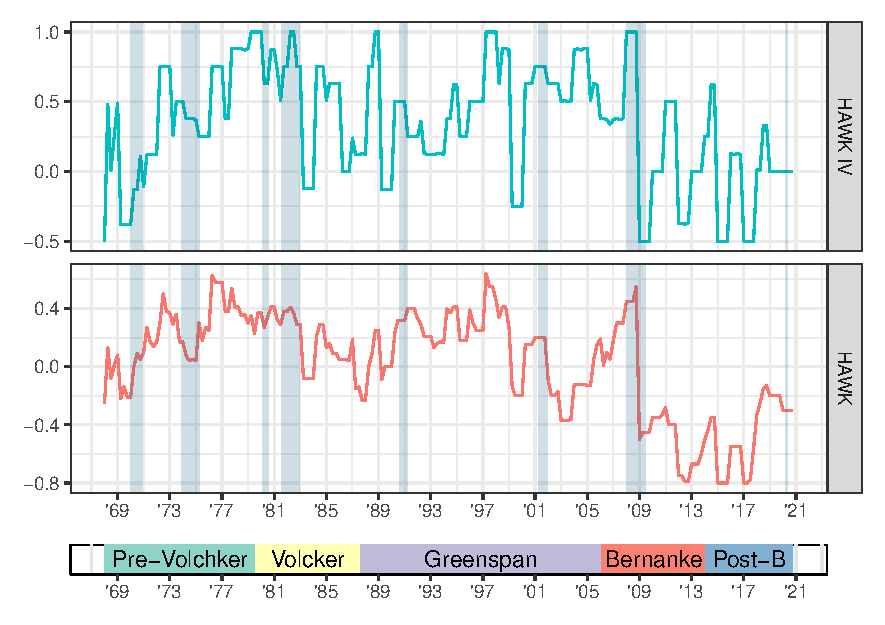
\includegraphics[width=0.8\textwidth]{HAWK_plot_w_heads.pdf}
    \end{figure}
\end{frame}




\section{Data}
\begin{frame}
    \frametitle{Contents}
    \tableofcontents[currentsection]
\end{frame}




% \begin{frame}{Summary Statistics}
    
% \end{frame}




\section{Results}
\begin{frame}
    \frametitle{Contents}
    \tableofcontents[currentsection]
\end{frame}



\begin{frame}{Results I}{Policy Response to Tealbook GDP Deflator Inflation and FOMC Hawkishness}


    \begin{figure}[!htbp]\centering
        \begin{minipage}{.9\textwidth}
          \caption{Policy Response to Inflation and FOMC Hawkishness. Short Specification}\vspace{1ex}
          \label{fig:LP_short}
          \begin{subfigure}[b]{0.495\textwidth}
              \centering
              \caption{Average Resp. to Projected CPI Inflation}
              \label{fig:LP_short:average_inflation}
              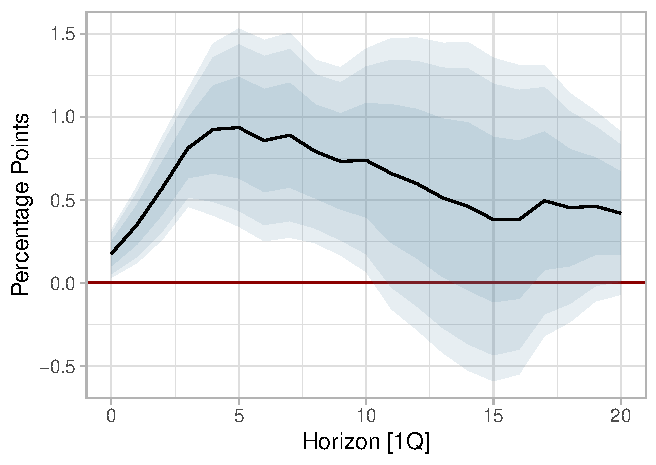
\includegraphics[width=\linewidth]{average_cpi_inflation_short.pdf}
          \end{subfigure}
          \hfill
          \begin{subfigure}[b]{0.495\textwidth}
              \centering
              \caption{Differential  Resp. to Projected CPI Inflation}
              \label{fig:LP_short:differential_inflation}
              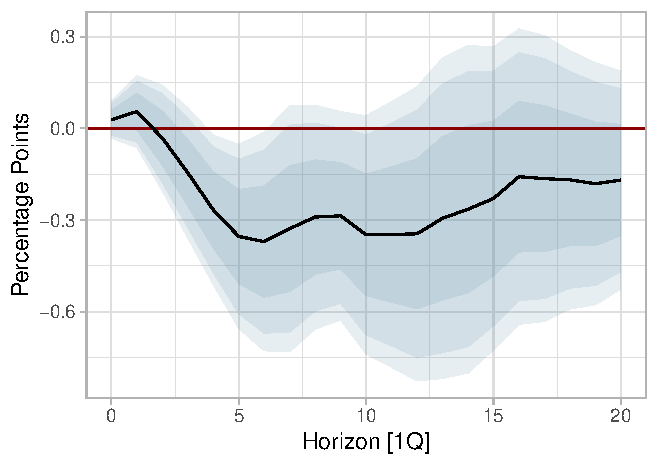
\includegraphics[width=\linewidth]{differential_cpi_inflation_short.pdf}
          \end{subfigure}\vspace{2ex}
          \begin{subfigure}[b]{0.495\textwidth}\centering
            \caption{Average Resp. to Projected GDP Gap}
            \label{fig:LP_short:average_gap}
            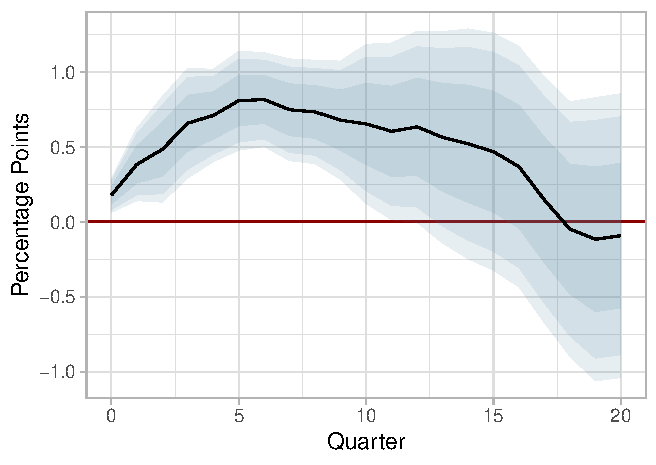
\includegraphics[width=\linewidth]{average_gap_short.pdf}
          \end{subfigure} \hfill
          \begin{subfigure}[b]{0.495\textwidth}\centering
            \caption{Differential Resp. to Projected GDP Gap}
            \label{fig:LP_short:differential_gap}
            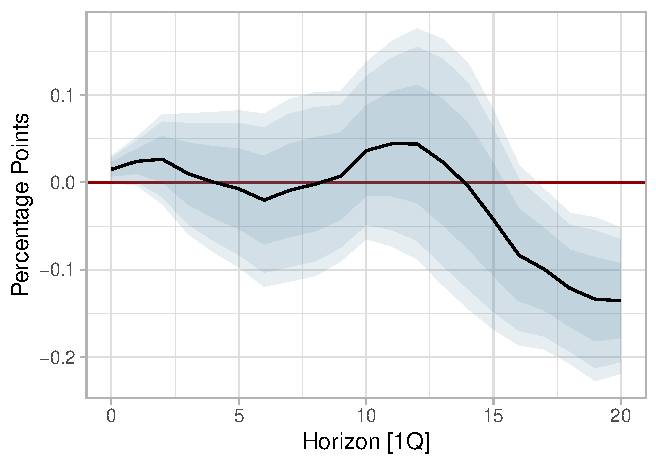
\includegraphics[width=\linewidth]{differential_gap_short.pdf}
          \end{subfigure}
              {\begin{flushleft}\scriptsize\textit{Notes}: This figure reports the responses of the $(r-r^*)_t$ to an increase in the Tealbook CPI inflation forecast and GDP gap forecast of 1 p.p. The subfigure \ref{fig:LP_short:average_inflation} reports the response of $(r-r^*)_t$ to projected CPI inflation for the $\mathit{HAWK}$ index equal to the sample average; \ref{fig:LP_short:differential_inflation} is the addition to the response in case there are 2 (out of 12 in total) additional consistent hawks in the FOMC. Subfigures \ref{fig:LP_short:average_gap} and \ref{fig:LP_short:differential_gap} report the same for the increase in projected GDP gap for 1p.p. The shaded areas correspond to 68\%, 90\% and 95\% confidence bands calculated with \citet{Andrews1991} HAC estimator.\end{flushleft}}
                  
        \end{minipage}
      \end{figure}
    
\end{frame}


\begin{frame}{Results I}{Policy Response to Tealbook Unemployment and FOMC Hawkishness}

    \begin{figure}[!htbp]\centering
        \label{fig:LP}
        \begin{subfigure}[b]{0.49\textwidth}
            \centering
            \caption{Average Response to Unempl. $\left(\beta_u^h\right)$}
            \label{fig:average_unemployment}
            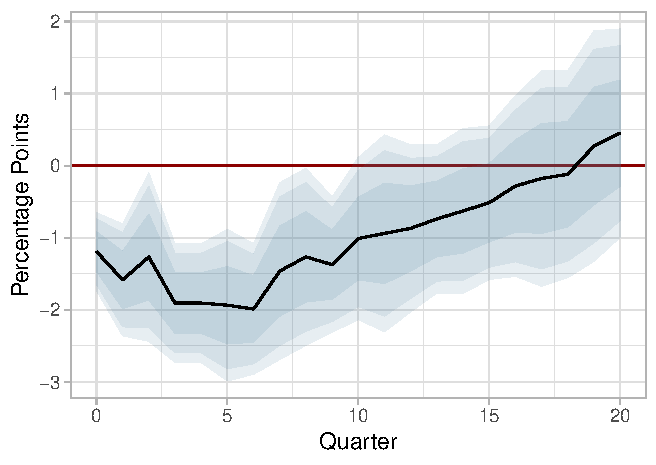
\includegraphics[width=\linewidth]{average_unemployment_longer.pdf}
        \end{subfigure}
        \hfill
        \begin{subfigure}[b]{0.49\textwidth}
            \centering
            \caption{Differential Response to Unempl. $\left(\gamma_u^h\right)$}
            \label{fig:differential_unemployment}
            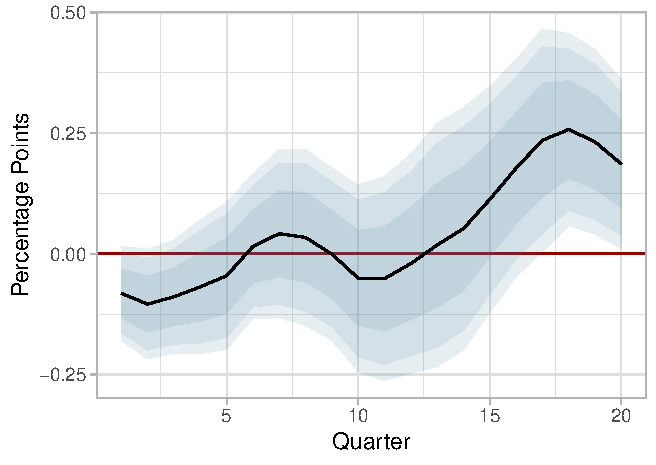
\includegraphics[width=\linewidth]{differential_unemployment_longer.pdf}
        \end{subfigure}\vspace{-4ex}
            {\begin{flushleft}\tiny\textit{Notes}: This figure reports the responses of the $r_t-\rho_t$ to an increase in the Tealbook unemployment forecast of 1 p.p. The subfigure \ref{fig:average_unemployment} reports the response for the $\mathit{HAWK}$ index equal to the sample average and \ref{fig:differential_unemployment} is the addition to the response in case there are 2 (out of 12 in total) additional consistent hawks in the FOMC. The shaded areas correspond to 68\%, 90\% and 95\% confidence bands calculated with Newey-West HAC estimator with Andrews-selected truncation parameter.\end{flushleft}}
    \end{figure}
    
\end{frame}


\begin{frame}{Results II}{Policy Response to Tealbook CIP Inflation and FOMC Hawkishness}

    \begin{figure}[!htbp]\centering
        \label{fig:LP2}
        \begin{subfigure}[b]{0.48\textwidth}
            \centering
            \caption{Average Response to Inflation $\left(\beta_\pi^h\right)$}
            \label{fig:average_inflation}
            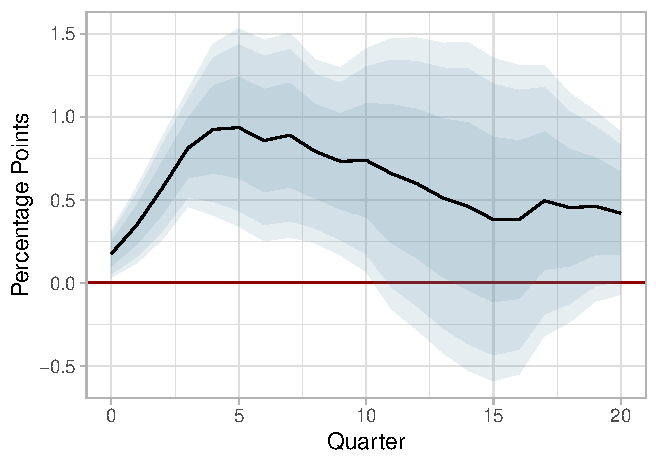
\includegraphics[width=\linewidth]{average_cpi_inflation_shorter.pdf}
        \end{subfigure}
        \hfill
        \begin{subfigure}[b]{0.48\textwidth}
            \centering 
            \caption{Differential Response to Inflation $\left(\gamma_\pi^h\right)$}
            \label{fig:differential_inflation}
            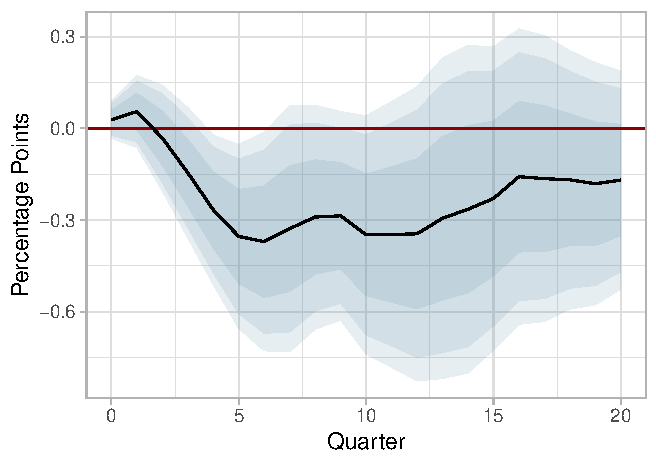
\includegraphics[width=\linewidth]{differential_cpi_inflation_shorter.pdf}
        \end{subfigure}\vspace{-4ex}
            {\begin{flushleft}\tiny\textit{Notes}: This figure reports the responses of the $r_t-\rho_t$ to an increase in the Tealbook inflation forecast of 1 p.p. (calculated as a predicted change in GDP deflator). 
            The subfigure \ref{fig:average_inflation} reports the response for the $\mathit{HAWK}$ index equal to the sample average and \ref{fig:differential_inflation} is the addition to the response in case there are 2 (out of 12 in total) additional consistent hawks in the FOMC. The shaded areas correspond to 68\%, 90\% and 95\% confidence bands calculated with Newey-West HAC estimator with Andrews-selected truncation parameter.\end{flushleft}}
    \end{figure}
    
\end{frame}


\begin{frame}{Results II}{Policy Response to Tealbook Output Gap and FOMC Hawkishness}

    \begin{figure}[!htbp]\centering
        \label{fig:LP}
        \begin{subfigure}[b]{0.49\textwidth}
            \centering
            \caption{Average Response to Output Gap $\left(\beta_u^h\right)$}
            \label{fig:average_unemployment}
            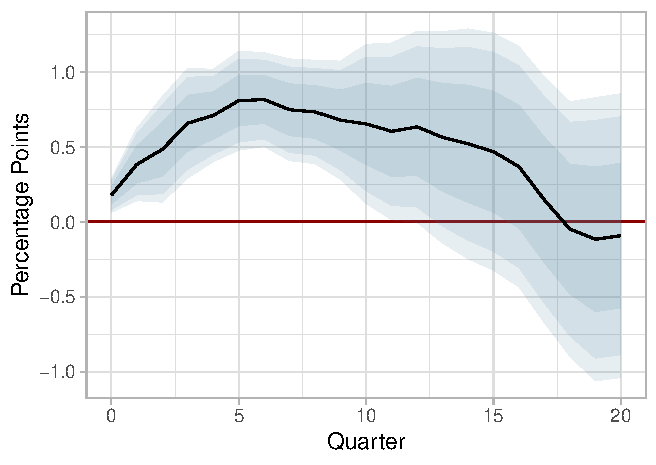
\includegraphics[width=\linewidth]{average_gap_shorter.pdf}
        \end{subfigure}
        \hfill
        \begin{subfigure}[b]{0.49\textwidth}
            \centering
            \caption{Differential Response to Gap $\left(\gamma_u^h\right)$}
            \label{fig:differential_unemployment}
            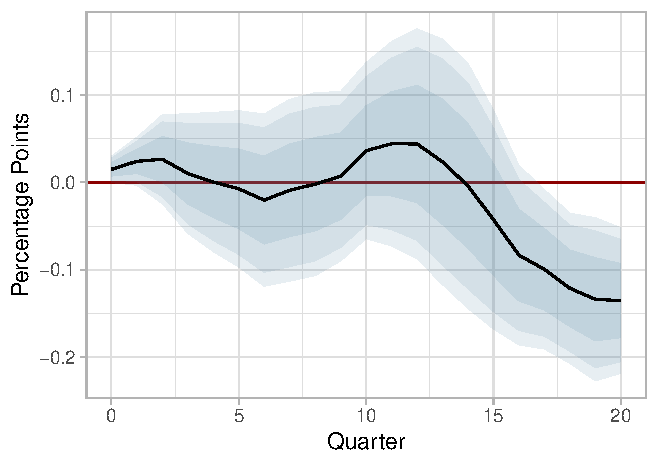
\includegraphics[width=\linewidth]{differential_gap_shorter.pdf}
        \end{subfigure}\vspace{-4ex}
            {\begin{flushleft}\tiny\textit{Notes}: This figure reports the responses of the $r_t-\rho_t$ to an increase in the Tealbook unemployment forecast of 1 p.p. The subfigure \ref{fig:average_unemployment} reports the response for the $\mathit{HAWK}$ index equal to the sample average and \ref{fig:differential_unemployment} is the addition to the response in case there are 2 (out of 12 in total) additional consistent hawks in the FOMC. The shaded areas correspond to 68\%, 90\% and 95\% confidence bands calculated with Newey-West HAC estimator with Andrews-selected truncation parameter.\end{flushleft}}
    \end{figure}
    
\end{frame}



\begin{frame}{Results}{Predicted IRFs}
    \begin{figure}[!htbp]\centering
        \begin{minipage}{\textwidth}
          \caption{Predicted IRFs in each of the state} 
          \label{fig:predicted_IRF}
          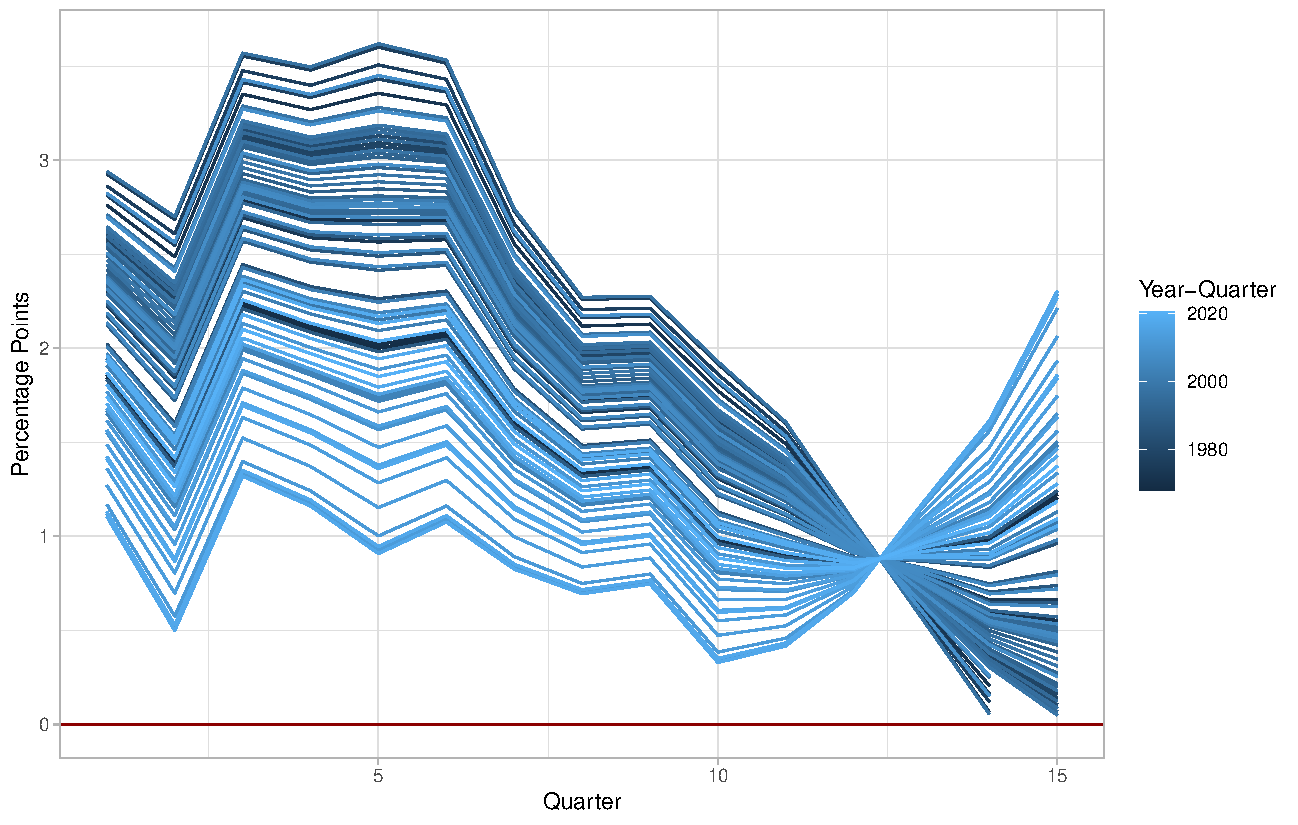
\includegraphics[width=0.5\linewidth]{irfs_plot_longer.pdf}%
          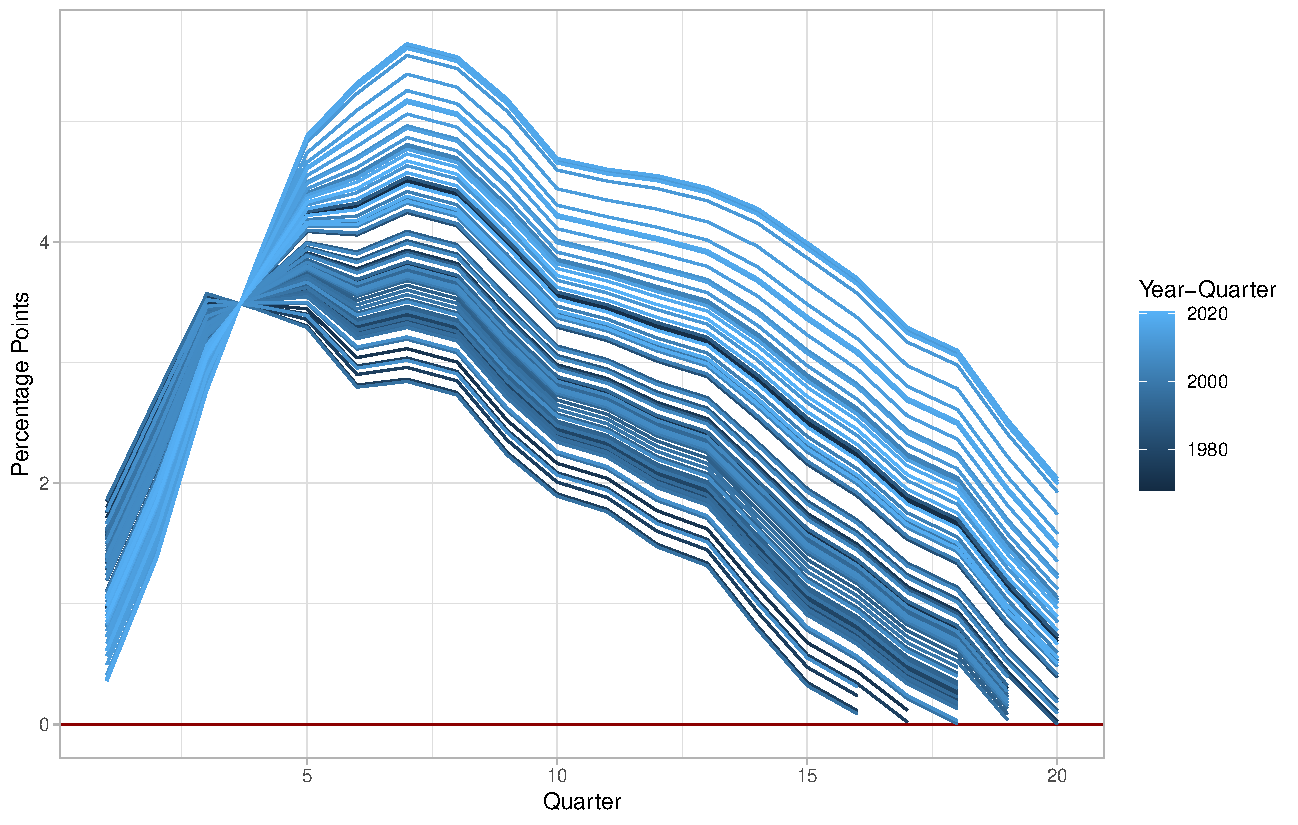
\includegraphics[width=0.5\linewidth]{irfs_plot_shorter.pdf}
          {\begin{flushleft}\tiny \textit{Notes:} This figure shows the Impulse Response functions in each state calculated as in equation \eqref{eq:InterestRatePath}.\end{flushleft}} 
          \end{minipage}
      \end{figure}
\end{frame}


\section{Size-Persistence Estimates}

\begin{frame}\frametitle{Size-Persistence in RANK}
    Rate path:
        \begin{equation*}
            r_t=\rho+e^{-\eta t}(r_0-\rho).\label{eq:InterestRatePath}
        \end{equation*}
    
    NK policy    
    \[C_0=\bar C\exp\left(-\frac{1}{\gamma}\int_0^\infty \left(r_s-\rho\right)\,ds\right).\]
    
    Size:
    \begin{equation*}
        R_0=\int_0^\infty \left(r_s-\rho\right)\,ds,\label{eq:KMVsize}
    \end{equation*}
    
    
    \[\frac{-d \log C_0}{dR_0}=\frac{1}{\gamma},\]
    
    
    \end{frame}
    
    \begin{frame}\frametitle{Picture of Size-Persistence trade-off}
        \begin{figure}\centering
            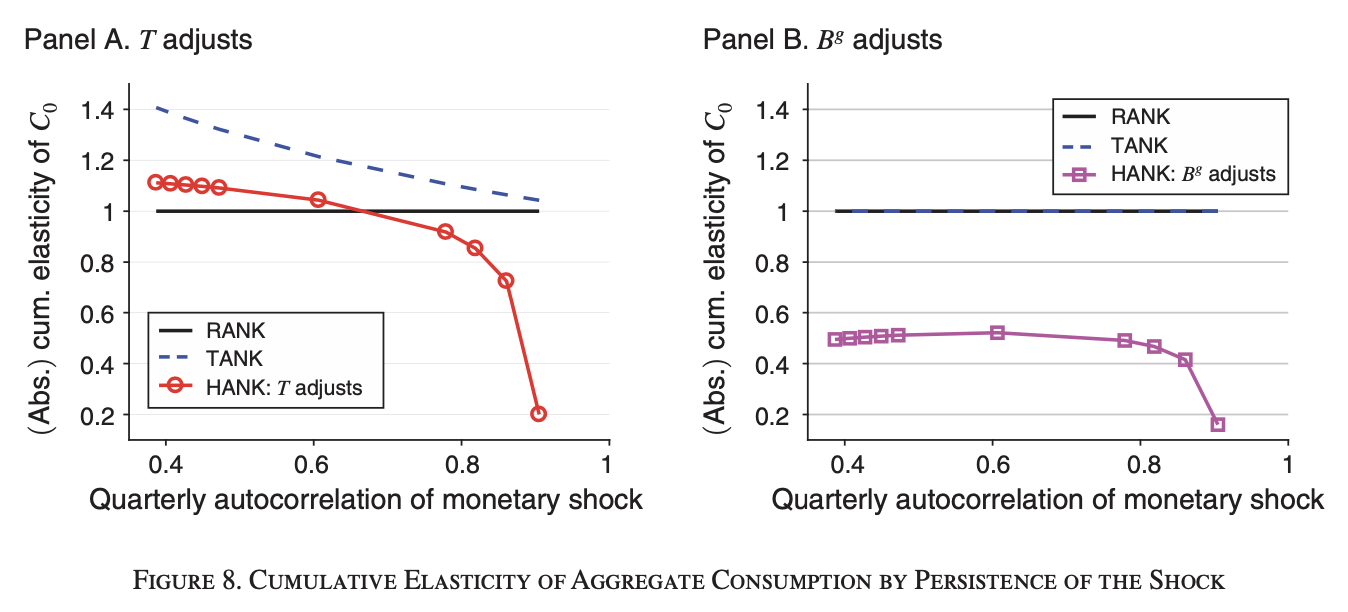
\includegraphics[scale=0.47]{Size_Persistence_KMV.png}
            \caption{The difference between the New Keynesian models from \citet{KMV2018}}
        \end{figure}
    \end{frame}
    
    
    \begin{frame}{Size-Persistent tradeoff by \citet{KMV2018}, formally}
        \begin{align}
            \textit{RANK:}&\quad& \frac{d}{d\nu}\frac{-d\log C_0}{dR_0}&=0     \label{eq:SizePersistenceRANK}\\
        \textit{TANK with $B^g$ adjustment:}&\quad& \frac{d}{d\nu}\frac{-d\log C_0}{dR_0}&= 0     \label{eq:SizePersistenceTANK_B}\\
        \textit{TANK with $T$ adjustment:}&\quad& \frac{d}{d\nu}\frac{-d\log C_0}{dR_0}&< 0     \label{eq:SizePersistenceTANK_T}\\
        \textit{HANK:}& \quad& 
            \frac{d^2}{d\nu ^2}\frac{-d\log C_0}{dR_0}&<0
            \label{eq:SizePersistenceHANK}
        \end{align}
        
    \end{frame}

\begin{frame}{Size-Persistence }{}
    \begin{figure}[!hpbt]\centering
        \begin{minipage}{0.8\textwidth}
          \caption{Estimates of Size and Persistence} 
          \label{fig:size_persistence}
          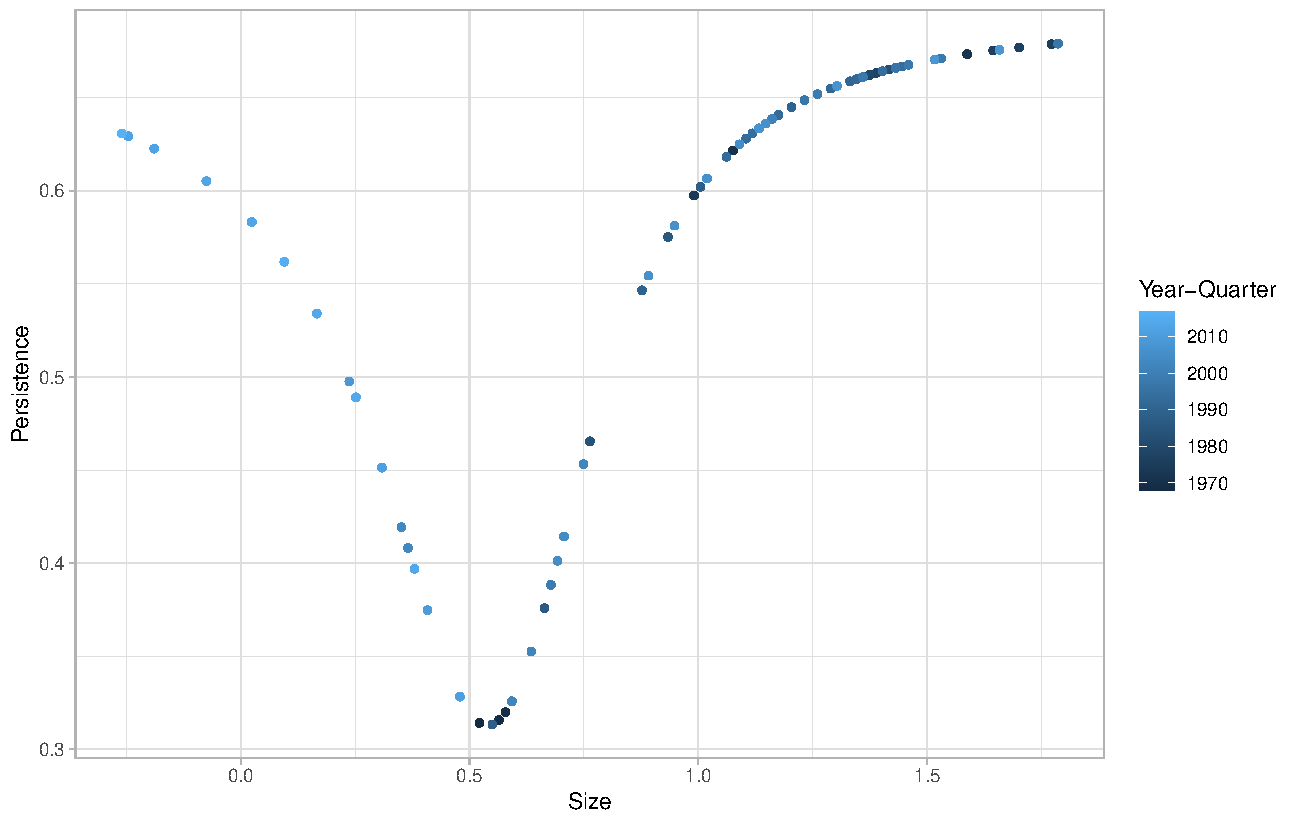
\includegraphics[width=\linewidth]{size_vs_persistence.pdf}
        %   {\begin{flushleft}\scriptsize \textit{Notes:} \end{flushleft}} 
          \end{minipage}
      
      \end{figure}
    
\end{frame}


\begin{frame}{Size and Persistence Over Time}
    \begin{figure}[!htbp]\centering
        \vspace{-2ex}
        \label{fig:Size_Persistence_Dynamics}
        \begin{subfigure}[b]{0.49\textwidth}
            \centering
            \caption{Size Dynamics}
            \label{fig:AverageResponce}
            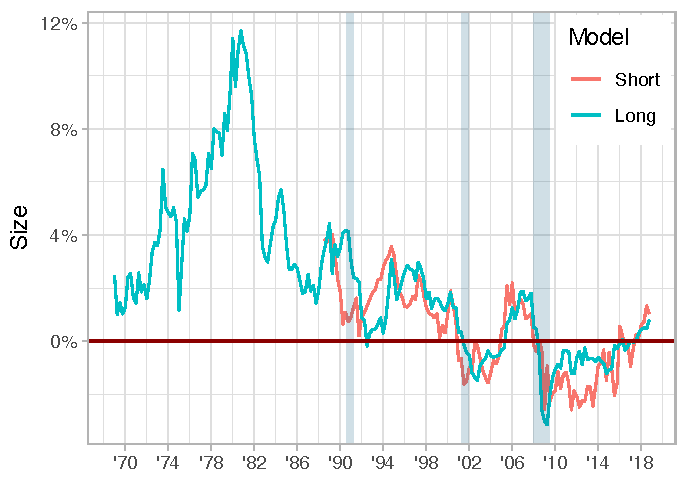
\includegraphics[width=\linewidth]{size_plot.pdf}
        \end{subfigure}
        \hfill
        \begin{subfigure}[b]{0.49\textwidth}
            \centering
            \caption{Persistence Dynamics}
            \label{fig:DifferentialResponce}
            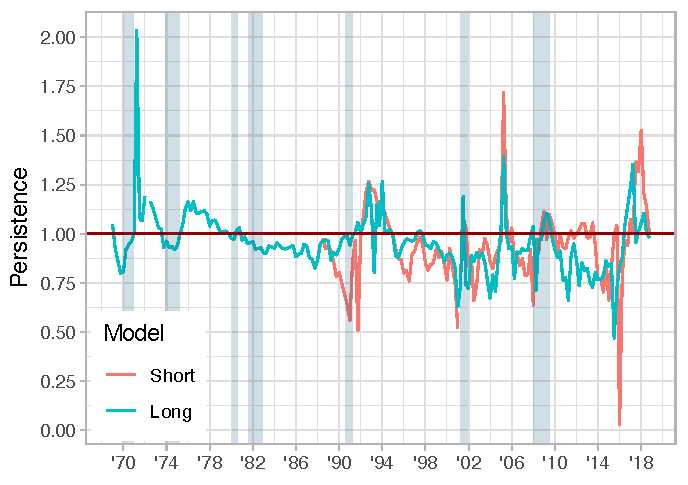
\includegraphics[width=\linewidth]{persistence_plot.pdf}
        \end{subfigure} \vspace{-5ex}
            {\begin{flushleft}\tiny\textit{Notes}: This figure presents the size and persistence, calculated as mean and the first autocorrelation of impulse-response function in each state, constructed as described in \vref{eq:InterestRatePath}, over time. \end{flushleft}}
      \end{figure}
      
\end{frame}







\section{Conclusion}
\begin{frame}\frametitle{Conclusions}
    \begin{block}{So, should we believe in HANK?}
        The evidence above suggests that, we should. 
        At least we have found that consumption behaviour in size-persistent tradeoff corresponds to the TANK model.
    \end{block}
\end{frame}





%Thanks
\begin{frame}

\begin{center}
    \Large Place for your suggestions and comments!
\end{center} 
\begin{center}
    \footnotesize
If you have any other suggestions/comments  please write \href{mailto://avlasov@nes.ru}{avlasov@nes.ru}
\end{center}


\end{frame}





\appendix
\section{Data}

\begin{frame}
    \frametitle{Apendixes}
    \tableofcontents[currentsection]
\end{frame}

\begin{frame}\frametitle{Data}
    \begin{itemize}\setlength\itemsep{1em}
        \item FED inflation (deflator, and CPI), GDP gap, unemployment forecast and NAIRU are from Tealbook (average of 1 and 2 quarter quarters ahead + averaging of FOMC meetings per quarter).
        \item HAWK index from \citet{HIM2023}.
        \item Natural rate of interest by \citet{HLW2017,HLW2023}
        \item Short-term rate ($r$) is by \citet{WuXia2016} and Fed Funds Rate 
        \end{itemize}
    \end{frame}

    \begin{frame}
        \begin{figure}[h!]\centering 
            \caption{Rates}\vspace{-4ex}
            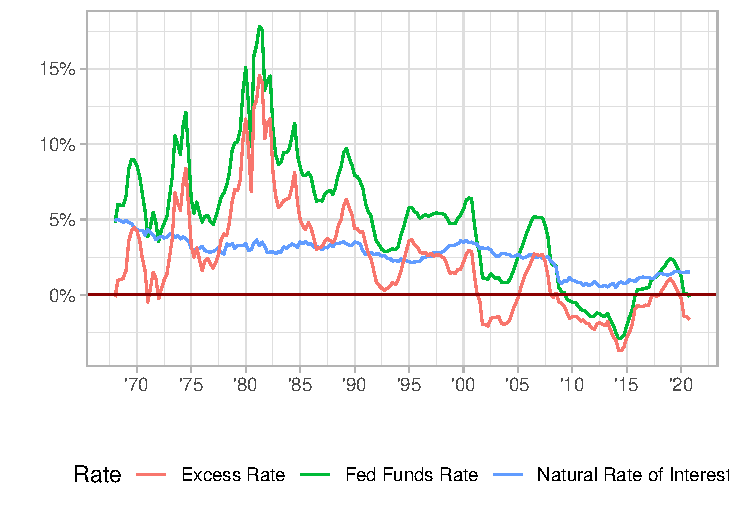
\includegraphics[width=.7\textwidth]{rate_plot.pdf}
        \end{figure}
    \end{frame}

    \begin{frame}
        \begin{figure}\centering
            \begin{subfigure}[b]{0.46\textwidth}\centering
            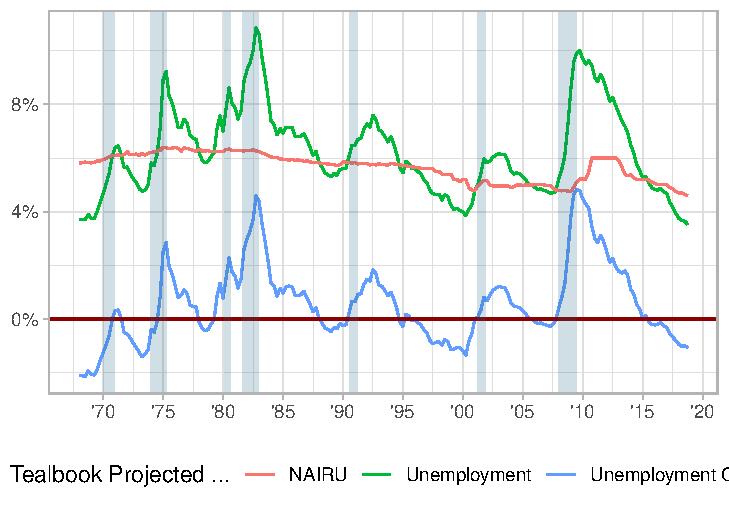
\includegraphics[width=\textwidth]{expected_unemployment_plot.pdf}
            \end{subfigure}%
            \begin{subfigure}[b]{0.46\textwidth}\centering
            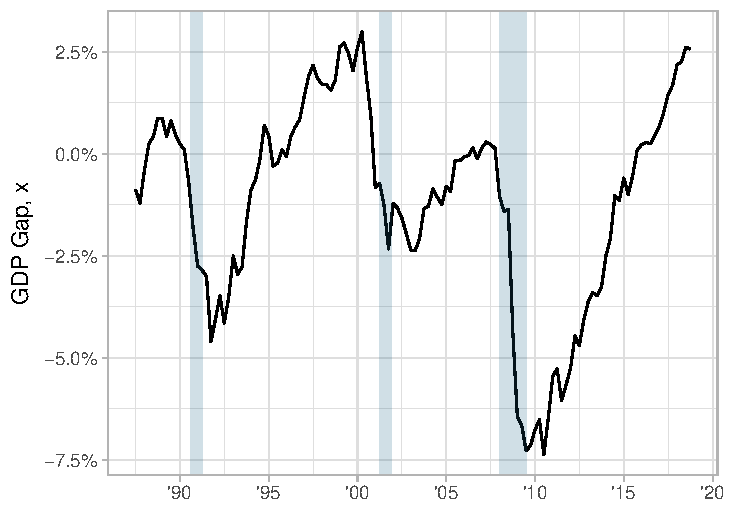
\includegraphics[width=\textwidth]{expected_gap_plot.pdf}
            \end{subfigure}
            \begin{subfigure}[b]{0.46\textwidth}\centering
            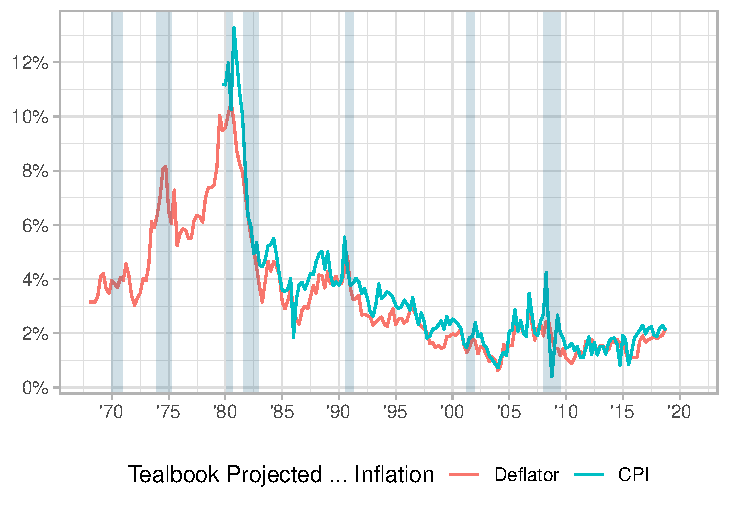
\includegraphics[width=\textwidth]{expected_inflation_plot.pdf}
            \end{subfigure}
        \end{figure}
    \end{frame}


\begin{frame}[t, allowframebreaks]
    \frametitle{References}
   \bibliography{../misc/references.bib}
    \bibliographystyle{../misc/econ.bst}
    \end{frame}
\end{document}